\section{Non-idealities of Forward Converter}

\subsection{Adding the Non-idealities and Their Solutions}

Firstly, we added the loss components of the MOSFET and the diodes. As we can see from the datasheet, MOSFET has $R_{ds,ON} = 12.4 m\ohm$, this value is added to the MOSFET. Then, the forward voltage values of the diodes are added to the software $V_f = 0.7V$ in our operation topology. After adding these, $R_{d,ON} = 1 m\ohm$ added for the diodes representing the losses on the selected diodes.

Series resistance of the inductor is given as maximum of $R_{max} = 0.113 \ohm$ for convenience we took this value as $0.6 \ohm$ to obtain an average operation range. Also, using the datasheet of the capacitor, we found out that the ESR value of the capacitor is around $3 m\ohm$. This is a low value, because the capacitor is a seramic capacitor and it has very low ESR operation.

Next step was to add the leakage inductances of the transformer, we have taken the leakage inductance as 1\% of the magnetizing inductance and introduced the leakage inductance as $13 \micro H$ to the primary side of the transformer.

Then it is very crucial to notice that the stored energy in the leakage inductance needs a way to decharge itself. For this very reason it is very important to design a snubber circuit around the MOSFET in order to block burnouts and have a smooth operation. We have decided to move on with a RC Snubber.

\begin{wrapfigure}{r}{0.5\textwidth}
  \vspace{-10pt}
  \begin{center}
    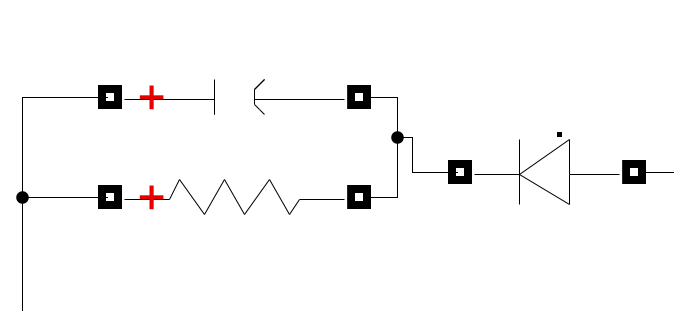
\includegraphics[width=0.4\textwidth]{Figs/snubberLay.PNG}
  \end{center}
  \vspace{-10pt}
  \caption{Snubber Layout}
  \label{Snubberlayout}
  \vspace{-10pt}
\end{wrapfigure}

When designing the RC snubber we can use an Application Note, in the application note, there is a snubber designed. We changed the R and C variables in order to adjust the solution into our problem. We have twice of voltage at the input and the current is twice. So, we used four times of R and two times of C. The values and the layout is in Figure \ref{Snubberlayout}:

$ R = 1250 \ohm$, $C=0.5 \micro F$


\subsection{Simulation of Non-ideal Case}

When we introduce all the non-idealities and run the simulation, the result is surprising. The output voltage waveform can be seen in Figure \ref{Output24non}

\begin{center}
\begin{figure}[H]
\centering
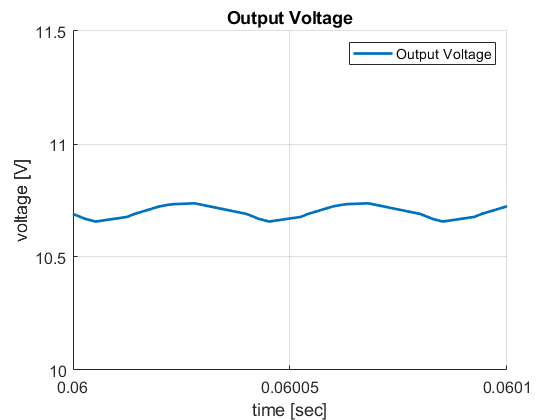
\includegraphics [width=12 cm, height= 8 cm]{output_voltage_non.png}
\caption{Output waveform of the forward converter 24V operation non-ideal}
\label{Output24non}
\end{figure}
\end{center}

We can see that due to the drops on the diodes, and the series parasitic resistances, the output voltage almost dropped to the $10.7V$. In order to compansate this value, we need to boost the duty cycle. We boost duty cycle to the 43.5\% for 24V operation.

\begin{center}
\begin{figure}[H]
\centering
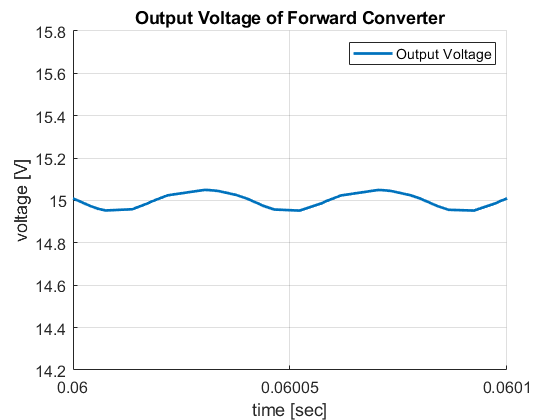
\includegraphics [width=12 cm, height= 8 cm]{output_voltage_com.png}
\caption{Output waveform of the forward converter 24V operation non-ideal}
\label{Output24com}
\end{figure}
\end{center}

\begin{figure}[H]
\centering
\begin{subfigure}{7 cm}
  \centering
  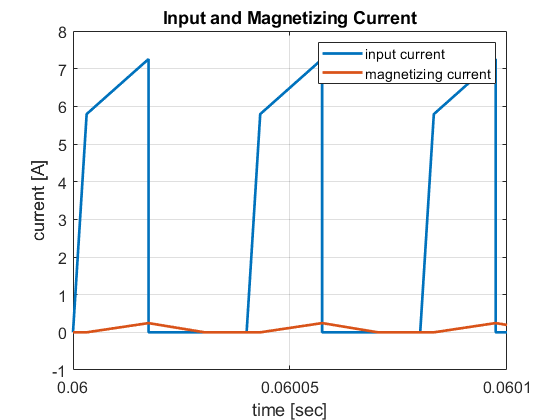
\includegraphics[width=7 cm]{Figs/input_current_24_com.png}
  \caption{Input and Magnetizing Current}
  \label{fig:input_current_24_com}
\end{subfigure}%
\begin{subfigure}{7 cm}
  \centering
  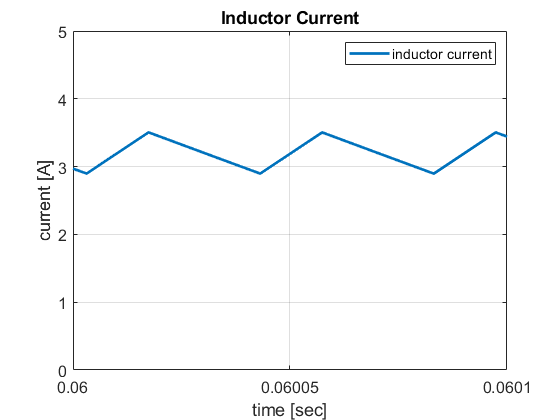
\includegraphics[width=7 cm]{Figs/inductor_current_com.png}
  \caption{Inductor Current}
  \label{fig:inductor_current_24_com}
\end{subfigure}
\caption{Forward converter input and inductor current under 24 non-ideal operation}
\label{fig:current_24}
\end{figure}

\begin{center}
\begin{figure}[H]
\centering
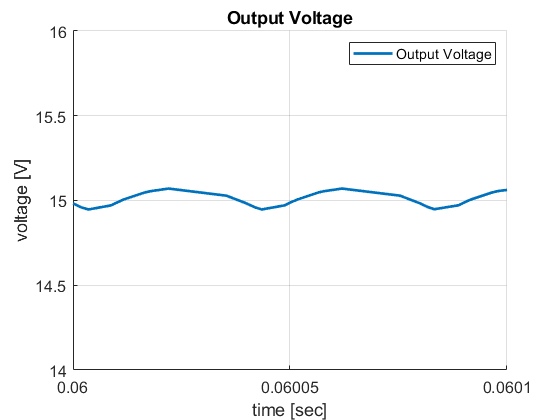
\includegraphics [width=12 cm, height= 8 cm]{output_voltage_non48.png}
\caption{Output waveform of the forward converter 48V non-ideal operation}
\label{Output48com}
\end{figure}
\end{center}

\begin{figure}[H]
\centering
\begin{subfigure}{7 cm}
  \centering
  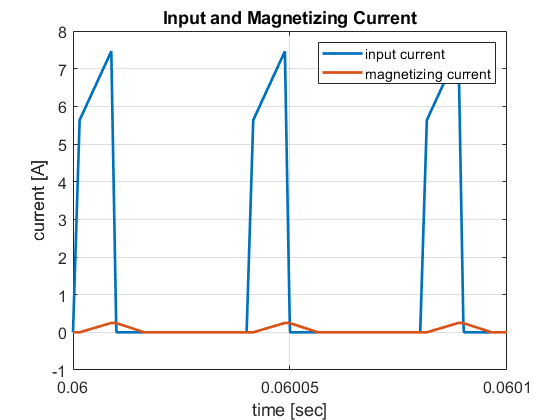
\includegraphics[width=7 cm]{Figs/input_current_non48.png}
  \caption{Input and Magnetizing Current}
  \label{fig:input_current_48_com}
\end{subfigure}%
\begin{subfigure}{7 cm}
  \centering
  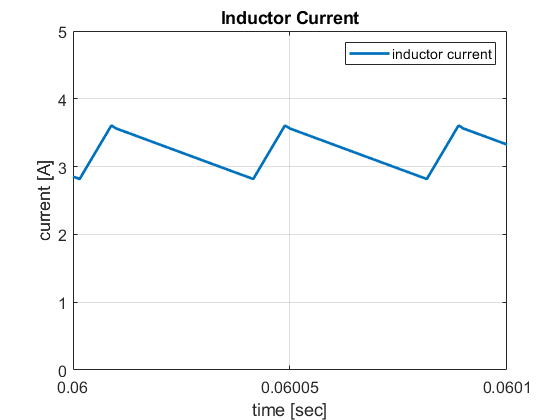
\includegraphics[width=7 cm]{Figs/inductor_current_non48.png}
  \caption{Inductor Current}
  \label{fig:inductor_current_48_com}
\end{subfigure}
\caption{Forward converter input and inductor current under 48V non-ideal operation}
\label{fig:current_24}
\end{figure}

The above simulations are for the non-ideal case with open-loop operation. Non-idealities drop the output voltage almost 2/3 of its value and decreases efficiency. Efficiency analysis will be done in the following parts.

In the ideal operations the duty cycles were calculated as: $D_{min} = 15.65\%$ and $D_{max} = 31.25\%$. However, in the non-ideal cases these values arised to higher values. So, it is very important to take non-idealities into account. This may result in inapplicable duty cycle values. Fortunately, our turn ratio decision $N=2$ is enough for non-ideal operation. Our non-ideal case duty cycles are:

$D_{min} = 22.05\%$, and $D_{max} = 43.5\%$

One of the most important parts is the snubber around the switch. We know that the leakage inductance of the transformer create high voltages around the switch and causes burn outs. We designed a snubber circuit and introduced it. The results of non-ideal switching with snubber is below:

\begin{figure}[H]
\centering
\begin{subfigure}{7 cm}
  \centering
  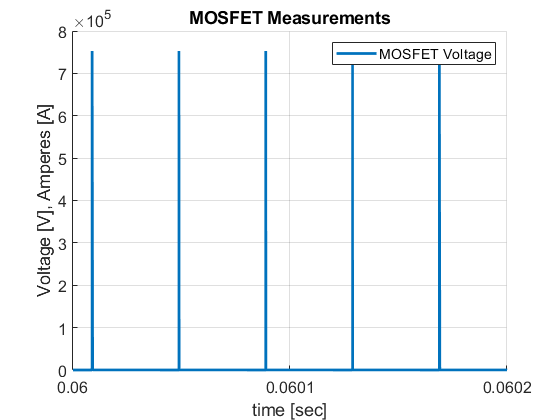
\includegraphics[width=7 cm]{Figs/nosnubber.png}
  \caption{MOSFET Voltage without Snubber}
  \label{fig:input_current_24_com}
\end{subfigure}%
\begin{subfigure}{7 cm}
  \centering
  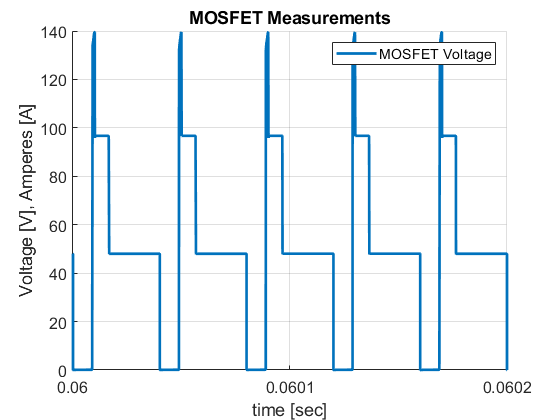
\includegraphics[width=7 cm]{Figs/snubber.png}
  \caption{MOSFET Voltage with Snubber}
  \label{fig:inductor_current_24_com}
\end{subfigure}
\caption{Snubber effect on the MOSFET operation with leakage inductance}
\label{fig:snubber}
\end{figure}

Since our MOSFET has a rated voltage of 150V, it is applicable. This snubber design is working.


